\documentclass[11pt]{article}

\usepackage[a4paper,margin=1.8cm]{geometry}
\emergencystretch=1em
\usepackage{graphicx}
\usepackage{array}
\usepackage{booktabs}
\usepackage{amsmath}
\usepackage{amssymb}
\usepackage{float}
\usepackage{subcaption}
\usepackage[hidelinks]{hyperref}
\usepackage{xurl}
\usepackage{caption}
\usepackage{enumitem}
\captionsetup{font=small,labelfont=bf}
\graphicspath{{../MT2026012/figures/}}

\usepackage{xcolor}
\usepackage{titlesec}
\usepackage{fancyhdr}
\definecolor{accent}{HTML}{8A5A2B}
\definecolor{sectionblue}{HTML}{1F4E5F}
\titleformat{\section}{\normalfont\Large\bfseries\color{sectionblue}}{\thesection}{0.6em}{}
\titleformat{\subsection}{\normalfont\large\bfseries\color{accent}}{\thesubsection}{0.6em}{}
\titleformat{\subsubsection}{\normalfont\normalsize\bfseries\color{accent}}{\thesubsubsection}{0.6em}{}
\titlespacing*{\section}{0pt}{3ex plus 0.5ex minus 0.3ex}{0.7ex plus 0.1ex}
\titlespacing*{\subsection}{0pt}{2.4ex plus 0.4ex minus 0.2ex}{0.5ex plus 0.1ex}
\titlespacing*{\subsubsection}{0pt}{1.9ex plus 0.3ex minus 0.2ex}{0.4ex}

\makeatletter
\renewcommand\@maketitle{%
  \newpage
  \null
  \vskip 1.2em%
  \begin{center}%
    {\LARGE \@title \par}%
  \end{center}%
  \par
  \vskip 2em}
\makeatother
\setlength{\headheight}{14pt}
\pagestyle{fancy}
\fancyhf{}
\fancyhead[C]{\color{accent}\rule{\textwidth}{0.8pt}}
\renewcommand{\headrulewidth}{0pt}
\renewcommand{\footrulewidth}{0.8pt}
\renewcommand{\footrule}{\color{accent}\hrule height 0.8pt}
\fancyfoot[C]{\thepage}

\title{\textbf{Machine Learning Course Project-I}\\[0.3em]
       \large Industrial Machine Condition Classification}
\date{}

\begin{document}
\maketitle

\section*{Team Name: Carrot}
\begin{center}
\small
\begin{tabular}{@{}>{\raggedright\arraybackslash}p{3.4cm}l>{\raggedright\arraybackslash}p{9.2cm}@{}}
\toprule
Name & Roll number & Contribution \\
\midrule
Aradhya Chakrabarti & MT2026012 & Preprocessing for the classification competition (data loading, cleaning and feature engineering); Models Tested: logistic regression (linear and quadratic), LDA, QDA, Gaussian naive Bayes, decision trees, random forests (with cross-validation, evaluation and hyperparameter tuning). Achieved the team's best public leaderboard score for the machine condition classification competition \\
Ankit Lamba & MT2026122 & Exploratory testing and data analysis for the flight competition; tested SVR, linear regression and random forest baselines \\
Kunal Yadav & MT2026047 & Ran preliminary prediction experiments for the flight competition \\
Kshitij Beri & MT2026046 & Implemented an ensemble model (blend) of trees, forests and boosting; achieved the team's best public leaderboard score on the flight competition \\
\bottomrule
\end{tabular}
\end{center}

\section*{Source code}
The full code for this competition is in the project repository: \url{https://github.com/TimeATronics/AIT511_Project1}

\section{Problem and dataset}

We are given a classification problem: classify a machine into one of three states using sensor measurements, with 0 for normal, 1 for thermal failure and 2 for mechanical failure. Thermal failures are driven by temperature and cooling conditions, and mechanical failures by load, wear, torque and vibration.

The training file \texttt{student\_dataset.csv} has 16,000 rows, and the test file has 4,000 rows. The columns are unit\_type (S/M/H) and ten sensors: ambient\_temp, process\_temp, coolant\_flow, shaft\_speed, drive\_torque, power\_load, component\_wear, thermal\_stress, mechanical\_load and vibration\_index. The column unit\_id identifies the machine (16,000 unique values, none of them in the test set) and is never used as a feature. The evaluation metric is accuracy.

We have used the following models: logistic regression (linear and quadratic basis), LDA, QDA, Gaussian naive Bayes, decision trees, and random forests, along with ensembles comprising of them and variations of the same.

\section{Data loading}

We load the three CSV files (training, test and the sample submission) with pandas. There are no duplicate rows, but every column has a small number of missing sensor readings, so we handle them during preprocessing and remove no rows.

\section{Exploratory data analysis}
\subsection{Class distribution}

For EDA, the first thing we check is the class balance, since an uneven split can make the accuracy higher than what the model is actually capable of. A count block and a bar plot show the classes are 8,000 / 4,000 / 4,000, that is a 2:1:1 split. A model that always predicts ``normal`` would already score 50\% accuracy, so we report balanced accuracy and metrics per class alongside accuracy later on while evaluating models.

\subsection{Sensor analysis by class}

Next we look at how the sensors behave for each class, since the failures are supposed to reflect the physics, that is, thermal problems should show up in temperature and stress variables, mechanical problems in wear, load and vibration. The code computes the sensor means per class and draws bar graph of means and boxplots (Figures~\ref{fig:machsensors} and~\ref{fig:machbox}). We check the average values per class below to see if that information can be observed in the data.

\begin{itemize}
  \item Thermal failures (class 1) are hotter: mean process\_temp 72.4 against 54.7 for normal and 62.2 for mechanical, and mean thermal\_stress 37.9 against 21.3 for normal.
  \item Mechanical failures (class 2) show more wear and load: mean component\_wear 165.0 against 87.4 for normal, mechanical\_load 88.0 against 64.8, and vibration\_index 2.10 against 1.51.
  \item Normal machines (class 0) have the lowest values of these variables, and the boxes for the two failure classes overlap the least exactly where the physical readings differ the most.
\end{itemize}

\begin{figure}[H]
\centering
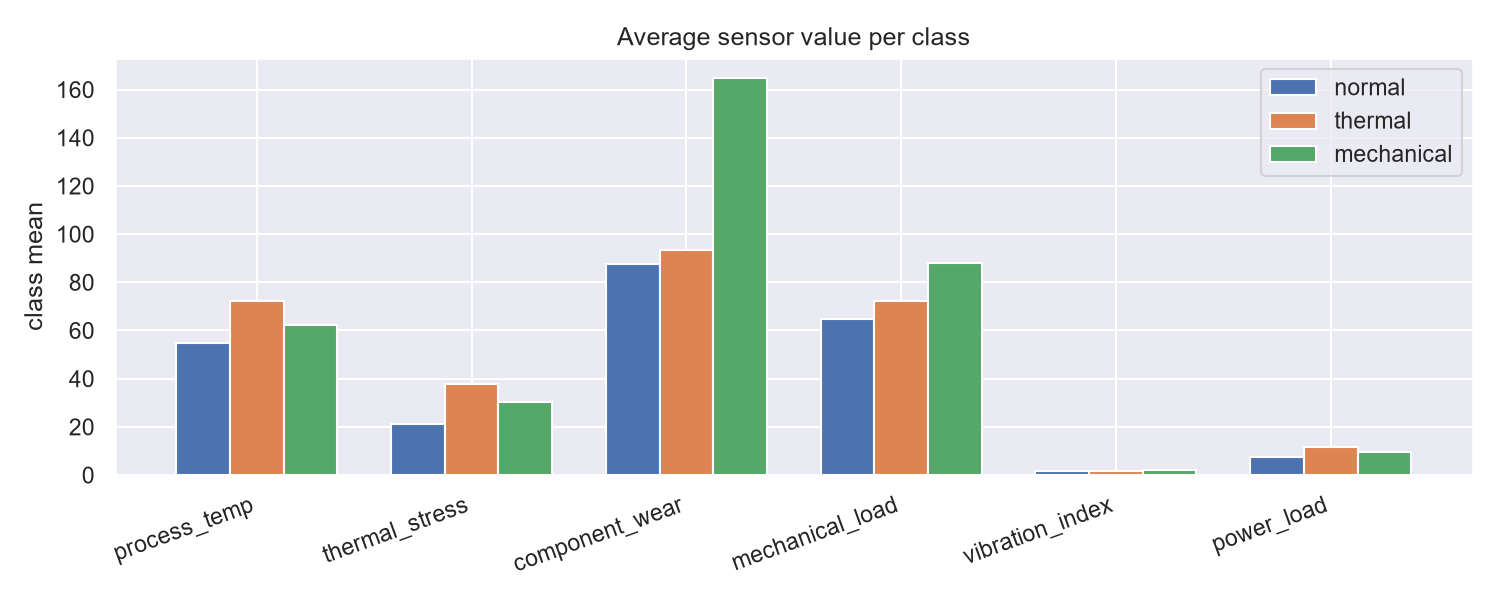
\includegraphics[width=0.82\linewidth]{machine_sensor_means.png}
\caption{Mean sensor readings per class for six key sensors.}
\label{fig:machsensors}
\end{figure}

\begin{figure}[H]
\centering
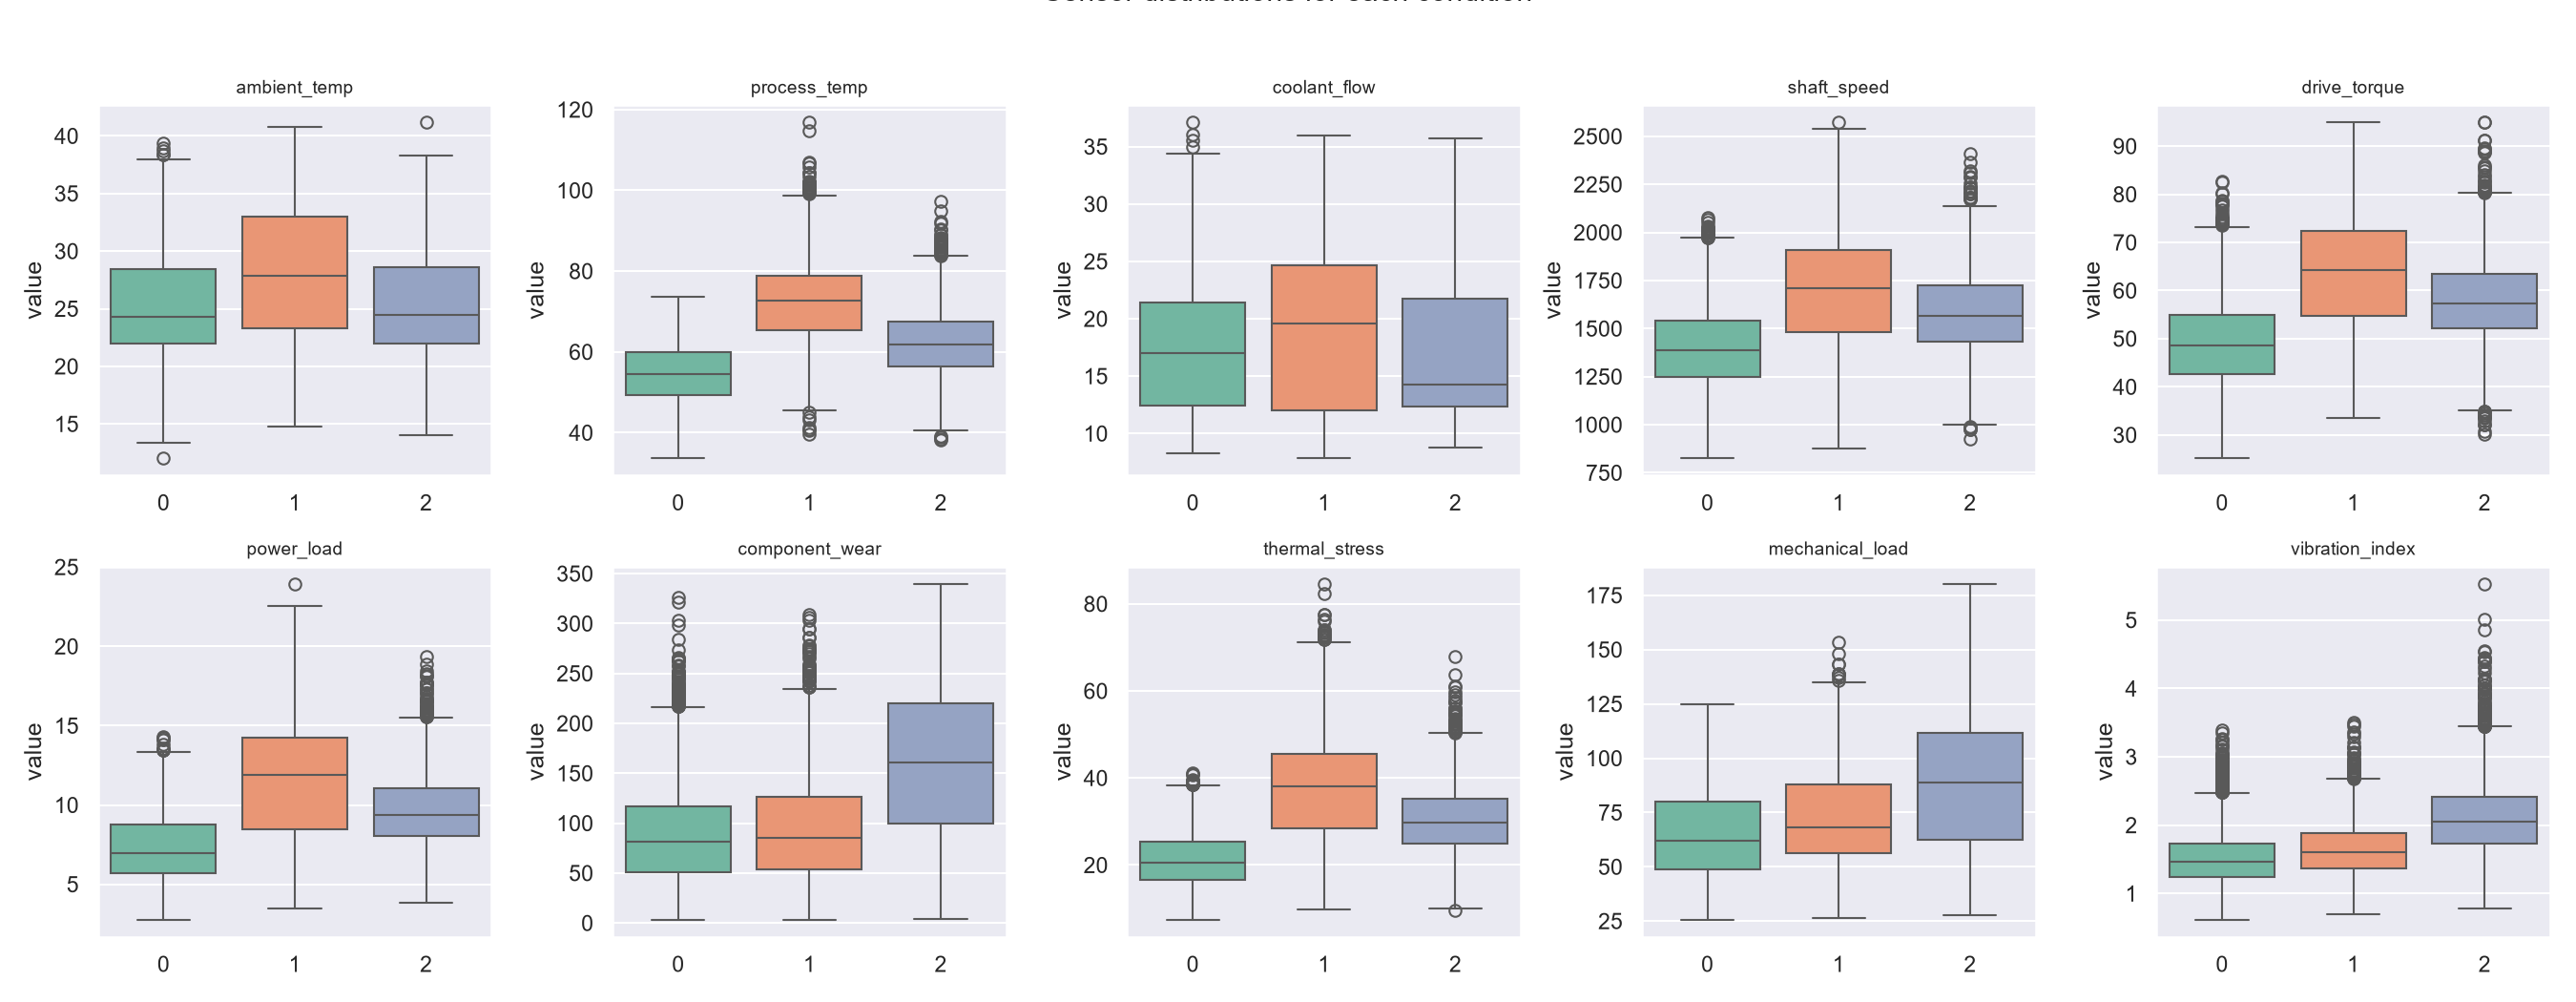
\includegraphics[width=\linewidth]{machine_boxplots_by_class.png}
\caption{Every sensor by class.}
\label{fig:machbox}
\end{figure}

\subsection{Missing value analysis}

We then check how many values are missing in each column, in order to decide how to fill them. The column with the most missing values is vibration\_index, which has 0.46\% of its values missing (74 rows), and the others fall between 0.14\% and 0.38\%. With numbers this small, filling the gaps with the column median is safe and no rows need to be dropped. unit\_type has 22 missing entries (0.14\%), which are filled with the most common type.

\subsection{Correlation analysis}

Next we check the correlations between the sensors, because they decide whether models that assume independent features are suitable. The heatmap block prints the strongest pairs as well. Fifteen pairs correlate above 0.5: the strongest are power\_load with thermal\_stress (0.93), drive\_torque with power\_load (0.92), and process\_temp with thermal\_stress (0.86). The sensors are therefore not really independent, which matters for the Naive Bayes classifier later.

\subsection{Machine type analysis}

Finally we check the machine type, since failure rates may depend on it. We observe that it is not neutral. 42.4\% of H machines are thermal failures, while S machines lean towards mechanical failures (29.4\%), so we retain type as a one-hot feature.

\section{Data cleaning}

There are no impossible values and no duplicate rows, so no rows are removed.

\section{Feature engineering}

Since the EDA showed that the two failure classes differ mainly in temperature and in wear and load, we add two kinds of extra features:

\begin{enumerate}
  \item \texttt{temp\_difference} $=$ process\_temp $-$ ambient\_temp. Thermal failures are driven by the machine being hotter than its surroundings.
  \item \texttt{power\_per\_speed} $=$ power\_load $/$ shaft\_speed, and \texttt{torque\_per\_wear} $=$ drive\_torque $/$ component\_wear. For cases where division by zero occurs, the imputer handles those as missing values.
\end{enumerate}

\section{Data preprocessing}

All preprocessing is done with a scikit-learn \texttt{ColumnTransformer} and used inside a \texttt{Pipeline}, so during cross-validation the transformations are fitted on the training folds only.

\begin{itemize}
  \item Missing values: the median for numeric columns, the most frequent value for unit\_type.
  \item Encoding: unit\_type is one-hot encoded, with \texttt{handle\_unknown="ignore"} in case the test set contains a type that training did not see.
  \item Scaling: standardisation for the models that need it (logistic regression, LDA, QDA, naive Bayes).
\end{itemize}

\section{Model evaluation}

The metric of the competition is accuracy, but as noted above, accuracy on its own can hide problems when the classes are uneven, so balanced accuracy and macro $F_1$ are recorded as well. For a two-class problem with predictions $\hat{y}$ and labels $y$,
\[
  \mathrm{precision} = \frac{\mathrm{TP}}{\mathrm{TP}+\mathrm{FP}}, \qquad
  \mathrm{recall} = \frac{\mathrm{TP}}{\mathrm{TP}+\mathrm{FN}}, \qquad
  F_1 = \frac{2\,\mathrm{precision}\,\mathrm{recall}}
            {\mathrm{precision}+\mathrm{recall}},
\]
and for the multi-class versions of these metrics, we can average these per-class values (macro $F_1$). Balanced accuracy is the average of the per-class recalls. It treats the three classes as equally important even when the split is 2:1:1. The ROC curve plots
\[
  \mathrm{TPR} = \frac{\mathrm{TP}}{\mathrm{TP}+\mathrm{FN}} \quad\text{against}\quad
  \mathrm{FPR} = \frac{\mathrm{FP}}{\mathrm{FP}+\mathrm{TN}},
\]
and the area under it (AUC) summarises the ranking quality across all thresholds.

For validation we split the training data into $K=5$ folds (maintaining the balance), and average the five scores: $\frac{1}{K}\sum_{k=1}^{K} e_k$. The final shortlisted models are re-checked with 5 folds repeated 3 times (15 scores each). A fixed random state (42) is used for every fold split and every model, to maintain reproducibility.

\section{Model family direct comparisons (baseline)}

We first train each model family once with reasonable settings:

\begin{itemize}
  \item \textbf{LDA}
  \item \textbf{QDA}
  \item \textbf{Gaussian naive Bayes}: independent Gaussian features per class, $p(x\mid y) = \prod_{j=1}^{d} p(x_j\mid y)$.
  \item \textbf{Logistic regression}: $\eta(x) = \sigma(w^\top x) = 1/(1+e^{-w^\top x})$.
  \item \textbf{Decision tree}: Recursive binary splitting with the Gini impurity, $\mathrm{Gini}(S) = 1 - \sum_k p_k^2$.
  \item \textbf{Random forest}: A majority vote across many decorrelated trees.
\end{itemize}

See Figure~\ref{fig:machinecomp}.

\begin{table}[H]
\centering
\small
\begin{tabular}{@{}>{\raggedright\arraybackslash}p{6.4cm}r@{}}
\toprule
Model & CV accuracy \\
\midrule
Random forest (300) & 0.8776 \\
QDA (raw sensors) & 0.8476 \\
Logistic regression (linear) & 0.8280 \\
LDA & 0.8239 \\
Decision tree (unrestricted) & 0.8056 \\
Gaussian naive Bayes & 0.7472 \\
\bottomrule
\end{tabular}
\caption{Baseline comparison of the model families.}
\label{tab:machbaseline}
\end{table}

We can observe that the random forest leads at 0.878, and QDA is the strongest of the three Gaussian models at 0.848. Plain logistic regression (0.828) and LDA (0.824) are below QDA because their boundaries are linear, and Gaussian naive Bayes is last at 0.747 because it assumes independent sensors while several pairs are correlated.

\begin{figure}[H]
\centering
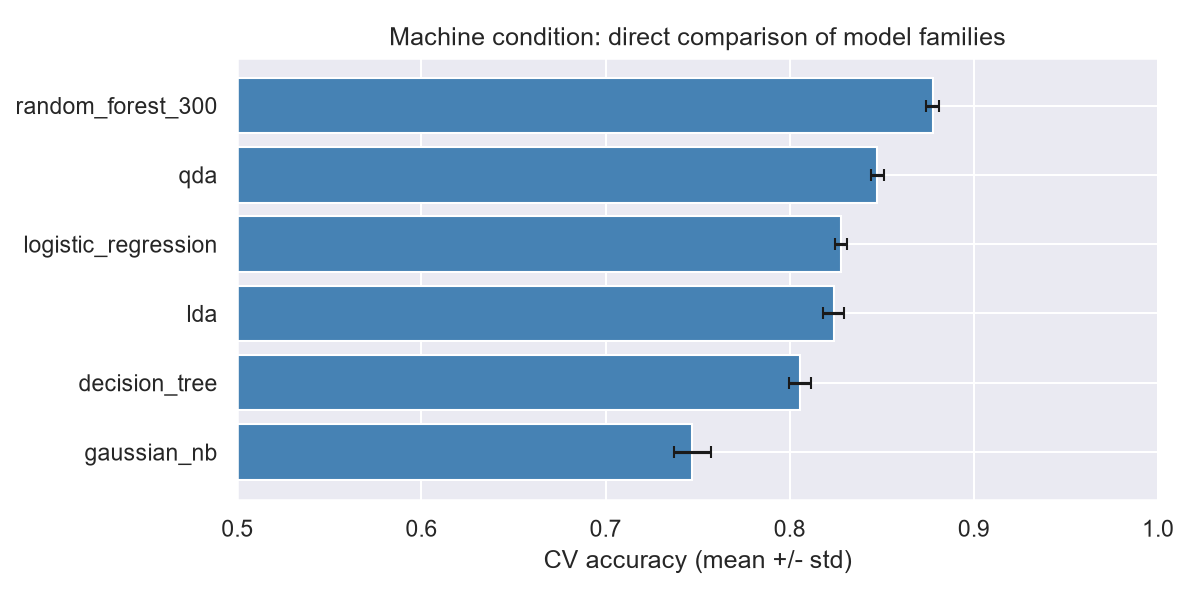
\includegraphics[width=0.78\linewidth]{machine_model_comparison.png}
\caption{Direct comparison of the model families (CV accuracy).}
\label{fig:machinecomp}
\end{figure}

\section{Hyper-Parameter Tuning}\label{sec:tuning}
\subsection{Logistic Regression (Linear): Regularisation Strength}

The strength is set through \texttt{C}, the inverse of the L2 penalty, and we iterate over it. The results are: $C=0.01$ gives accuracy 0.818, $C=0.1$ gives 0.825, $C=1$ gives 0.828, $C=10$ gives 0.829 and $C=100$ gives 0.829. Accuracy rises up to $C=10$ and stays flat. Hence we can see that a weaker penalty coefficient is better.

\subsection{Logistic Regression with a Quadratic Basis}

Since the boundaries in this dataset are not linear, we give the linear model squared and interaction terms of the sensors. This provides a quadratic boundary, using a pipeline with \texttt{PolynomialFeatures} at degree 2 before the logistic model. We try degree 1 versus 2 and $C \in \{0.01,0.1,1,10\}$. Degree 2 with $C=1$ reaches 0.8853, clearly above the linear version (0.829).

\subsection{QDA: Covariance Regularisation}

A small regularisation is added to each covariance, which keeps them invertible when the features are strongly related (singular matrices). When we do not add a regularization parameter, that is, \texttt{reg\_param} $=0$ the code crashes because \texttt{temp\_difference} is an exact linear combination of two sensors and the class covariance is singular. With regularisation, the QDA model shows accuracy of 0.8393, but it is below the previous accuracy of 0.8476 obtained from the raw sensors at \texttt{reg\_param} $=0.1$. Hence we continue using the raw-sensor version for QDA.

\subsection{Gaussian Naive Bayes: Variance Smoothing}

The Naive Bayes classifier assumes the sensors are conditionally independent given the class and adds a small smoothing value to every variance. We iterate over the smoothing value from $10^{-9}$ to $0.1$. The best setting (0.1) increases the score from 0.747 to 0.754 (still far lower than the rest).

\subsection{Decision Tree: Pre-pruning and Post-pruning}

For pre-pruning we tune four early stopping criteria: maximum depth, minimum leaf size, minimum samples needed to split a node, and the maximum number of leaves. The best pre-pruned tree has depth 12 with a minimum leaf size of 5 and scores 0.8389. The unrestricted tree falls to 0.806, and depth-4 trees underfit around 0.772. For post-pruning we use the cost-complexity criterion
\[
  R_\lambda(T) = R(T) + \lambda |T|,
\]
with candidate $\lambda$ values from the pruning path. Here post-pruning helps: the best $\lambda$ (about $3\times10^{-4}$, keeping 161 leaves) increases the cross-validation accuracy of the tree from 0.8389 to 0.8429 (Figure~\ref{fig:machprune}), while larger $\lambda$ values remove useful branches.

\begin{figure}[H]
\centering
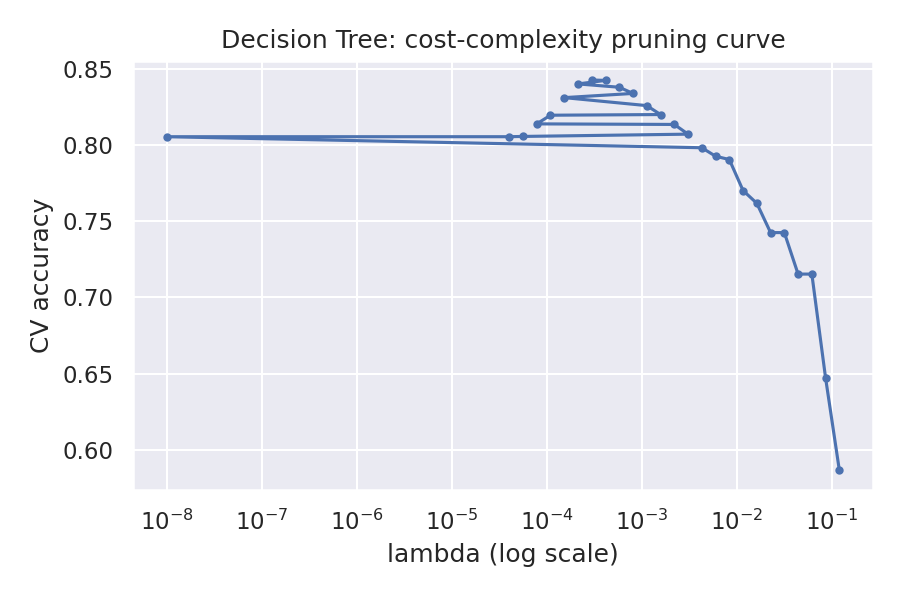
\includegraphics[width=0.56\linewidth]{machine_tree_pruning.png}
\caption{Cost-complexity pruning curve for the classification tree.}
\label{fig:machprune}
\end{figure}

\subsection{Random forest}

We tune the depths per tree, the minimum leaf size and the class weighting. We include class weights because the classes are split 2:1:1. The unweighted depth-14 random forest is the best at 0.8787, but the differences inside the unweighted block are tiny (0.876 to 0.879). Every \texttt{balanced} variant scores lower than the corresponding unweighted versions.

\section{Experiment: Class Imbalance Handling}

Since the 2:1:1 split could in principle hurt the two failure classes even while accuracy looks fine, we compare three approaches further on the two best models seen so far (the quadratic logistic regression and QDA): (i) reweighting the classes, (ii) random oversampling of the minority classes, and (iii) SMOTE, which creates synthetic minority samples by interpolating between neighbours.

\begin{table}[H]
\centering
\caption{Imbalance strategies for the quadratic logistic (5-fold CV).}
\label{tab:imbalance}
\small
\begin{tabular}{@{}lrr@{}}
\toprule
Variant & Accuracy & Macro $F_1$ \\
\midrule
none & 0.8853 & 0.8756 \\
reweight (class weights) & 0.8743 & 0.8666 \\
random oversampling & 0.8728 & 0.8649 \\
SMOTE & 0.8734 & 0.8660 \\
\bottomrule
\end{tabular}
\end{table}

Each of these experiment scenarios lowered both metrics. With classes that are already well separated and only a 2:1:1 split, the resampled training set biases the boundary towards synthetic or duplicated minority points without improving any real case, so we continue using the previous models only.

\section{Experiment: Combining/Blending the Top Models}

The two strongest single models seen so far are the quadratic and the cubic logistic regressors. We further tried using a cubic basis with stronger regularisation (degree 3, $C=0.3$), which reached an accuracy of 0.8894 $\pm$ 0.0031 under cross-validation, just above the quadratic model. We also tested three soft-voting combinations of the pair (considering a combination with the random forest in the third variant): The three variants are (i) an even 50/50 vote, (ii) a 60/40 vote weighted toward the quadratic model, and (iii) a 40/40/20 vote with the random forest. Each combination is scored with the same 5-fold cross-validation as everything else before.

\begin{table}[H]
\centering
\small
\setlength{\tabcolsep}{6pt}
\begin{tabular}{@{}>{\raggedright\arraybackslash}p{6.2cm}rrr@{}}
\toprule
Combination & Accuracy & Balanced acc. & Macro $F_1$ \\
\midrule
Quadratic 40\% + cubic 40\% + forest 20\% & 0.8919 & 0.8746 & 0.8828 \\
Quadratic 50\% + cubic 50\% & 0.8909 & 0.8738 & 0.8819 \\
Quadratic 60\% + cubic 40\% & 0.8901 & 0.8730 & 0.8810 \\
\bottomrule
\end{tabular}
\caption{The three probability-vote combinations under 5-fold cross-validation.}
\label{tab:machvotes}
\end{table}

All of these three combinations performed better than all previous models used by us so far. As per the public leaderboard scores, the 60/40 vote performs best at 0.89125, followed by the 40/40/20 vote (0.89062) and the even vote (0.89000), hence it is our best model.

\section{An 80/20 test of the best model}

We also test the best model and its strongest single-model member on an 80/20 split of the training data. This shows us how the models behave on rows they have never seen, and how much they still depend on the amount of training data.

\begin{table}[H]
\centering
\small
\setlength{\tabcolsep}{6pt}
\begin{tabular}{@{}>{\raggedright\arraybackslash}p{4.6cm}lrrr@{}}
\toprule
Model & Training rows & Accuracy & Balanced acc. & Macro $F_1$ \\
\midrule
Soft vote (60/40) & 80\% & 0.9003 & 0.8854 & 0.8921 \\
Soft vote (60/40) & 20\% & 0.8928 & 0.8763 & 0.8834 \\
Quadratic logistic & 80\% & 0.8953 & 0.8798 & 0.8862 \\
Quadratic logistic & 20\% & 0.8872 & 0.8731 & 0.8782 \\
\bottomrule
\end{tabular}
\caption{Scores of the best model and the quadratic logistic on the unseen 20\% of the training data.}
\label{tab:machholdout}
\end{table}

\begin{figure}[H]
\centering
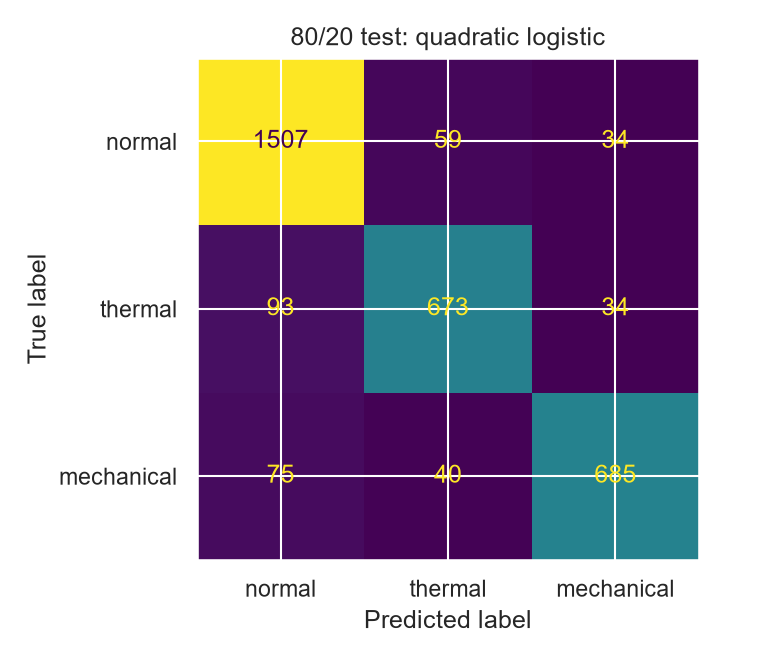
\includegraphics[width=0.42\linewidth]{machine_80_20_confusion.png}
\caption{Confusion matrix of the best model on the unseen 20\% of the training data.}
\label{fig:machholdoutconf}
\end{figure}

When we train the ensemble model on 80\% of the rows it scores 0.9003 on the 20\% remaining, and still 0.8928 from just 20\%, so the decision boundary is stable and does not depend upon data volume; The quadratic logistic model also has similar, but slightly lower metrics.

\section{Model Diagnostics}

\paragraph{Confusion matrices.} We compute out-of-fold predictions for the three leading models and draw their confusion matrices (Figure~\ref{fig:machconf}), with labels 0 normal, 1 thermal, 2 mechanical. With all the models, normal machines are recognised best (7,498 of 8,000 for the quadratic logistic). The two failure classes each have between 660 and 670 misclassifications, and most of those misses fall into the normal class, roughly 470 to 480 per class. Only about 180 to 200 machines, upon classification, get swapped between thermal and mechanical, and those two classes are the ones whose sensor boxes overlap the most.

\begin{figure}[H]
\centering
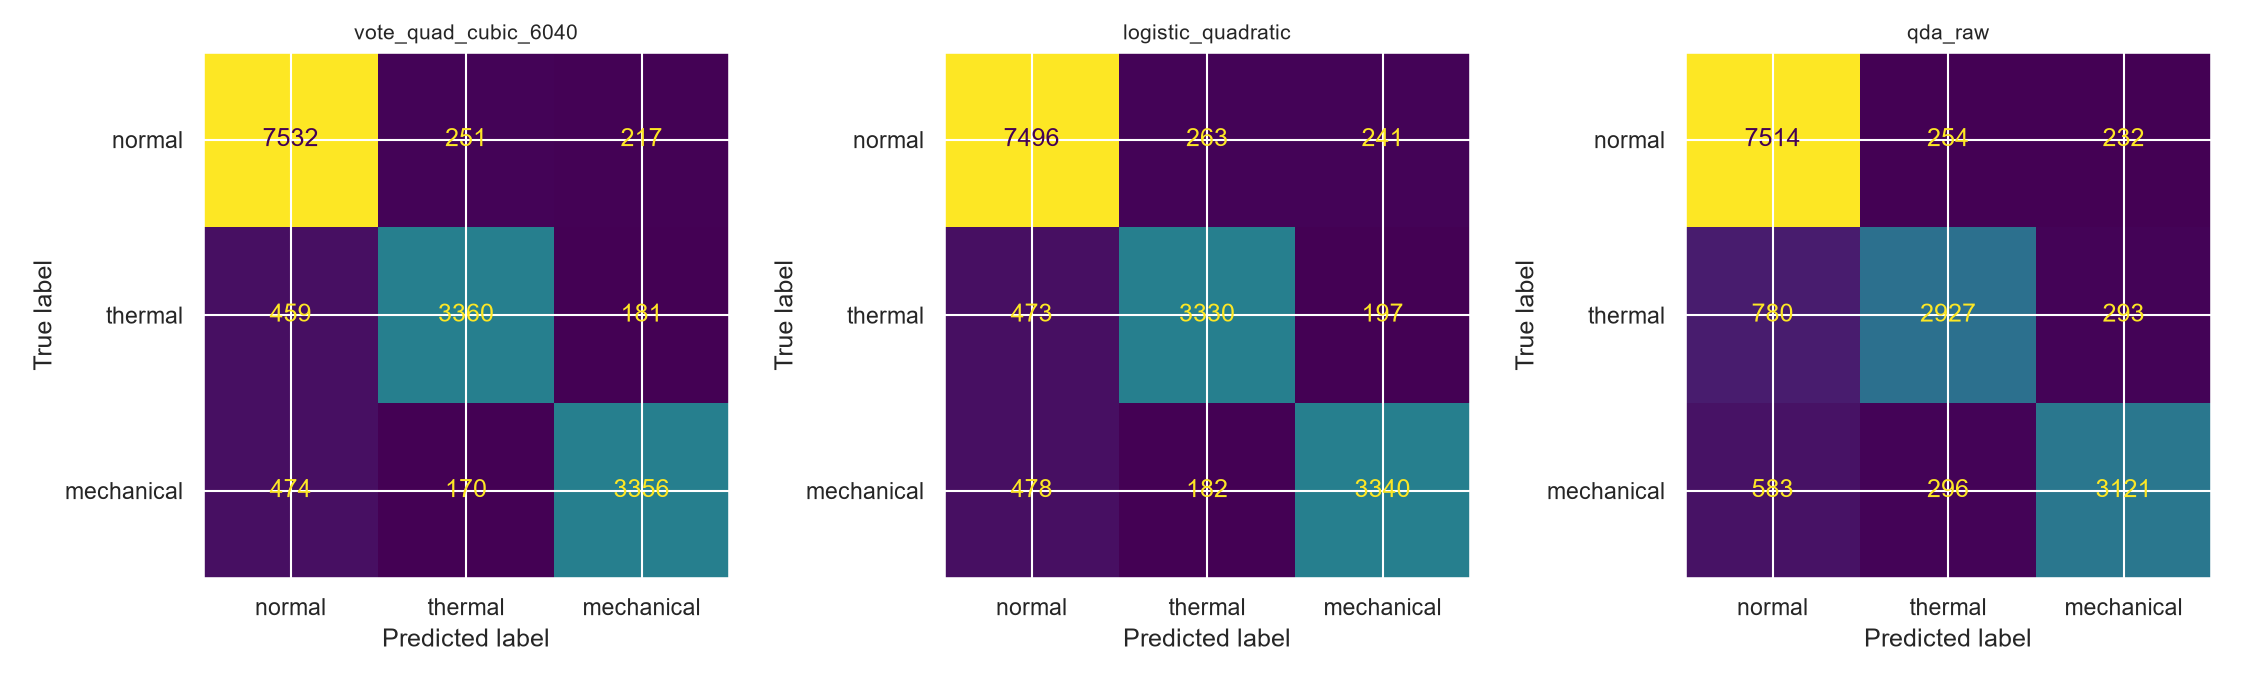
\includegraphics[width=\linewidth]{machine_confusion_matrices.png}
\caption{Out-of-fold confusion matrices for the three leading models.}
\label{fig:machconf}
\end{figure}

\paragraph{Per-class metrics.} We then print the full classification report for the quadratic logistic regression. Recall is 93.7\% on normal, 83.3\% on thermal and 83.5\% on mechanical, with precision and $F_1$ following closely. No class collapses, and the weakest recall is still above 80\%.

\paragraph{ROC curves.} Next we draw one-vs-rest ROC curves from the out-of-fold class probabilities and print the area under each curve. The two have almost identical overall discrimination (macro AUC 0.967 for the 60/40 vote against 0.966 for the quadratic logistic). The curves tend to go towards the top-left corner, and in both cases the thermal class has the highest AUC (0.972 for the 60/40 vote, 0.971 for the quadratic logistic).

\paragraph{Balanced metrics.} Finally we compute accuracy, balanced accuracy and macro $F_1$ for the three models and plot them side by side (Figure~\ref{fig:machbal}). The 60/40 vote-based ensemble model is best on all three metrics (0.8905, 0.8735 and 0.8814), the quadratic logistic model follows (0.8854, 0.8682 and 0.8757) and QDA is the worst out of these three.

\begin{figure}[H]
\centering
\begin{subfigure}{0.55\linewidth}
  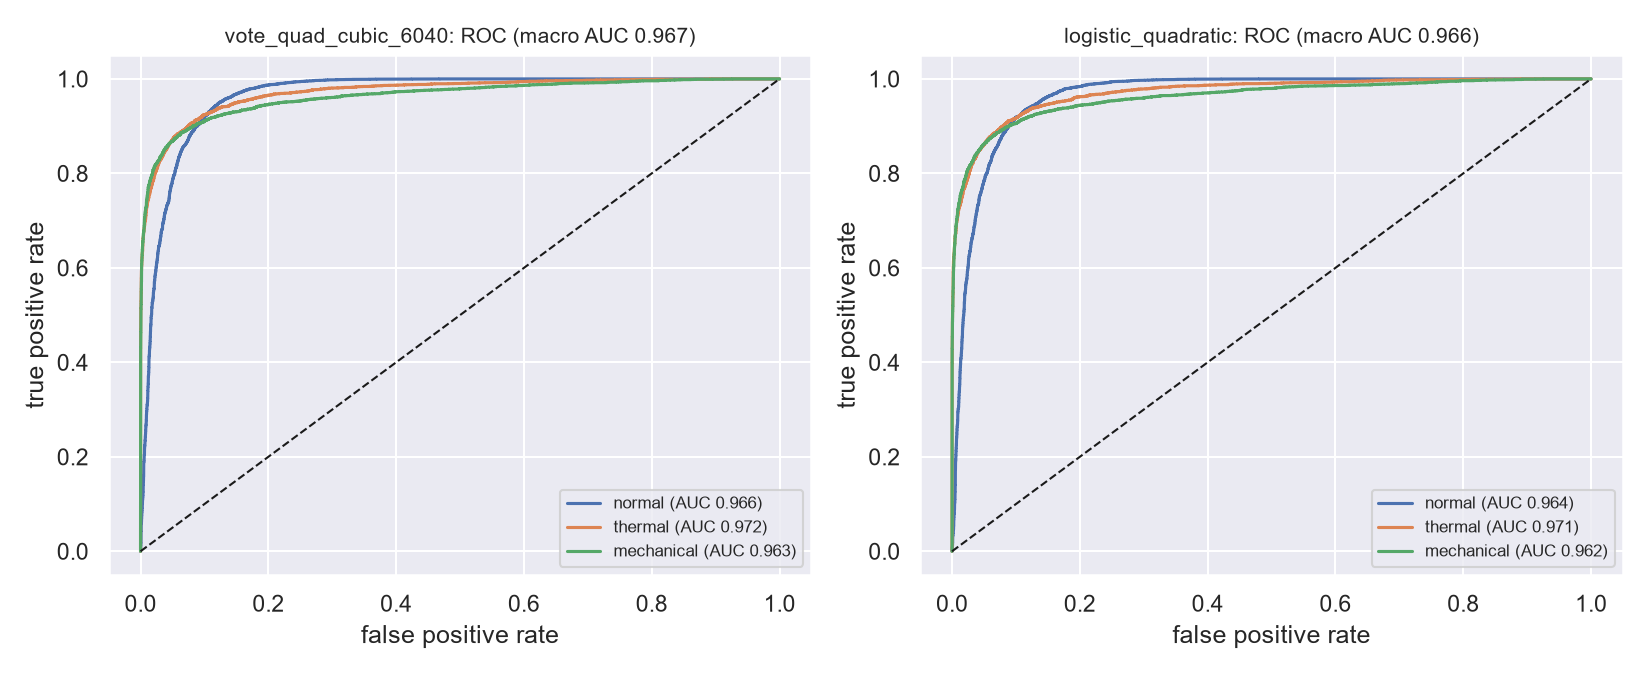
\includegraphics[width=\linewidth]{machine_roc_curves.png}
  \caption{one-vs-rest ROC}
\end{subfigure}
\hfill
\begin{subfigure}{0.42\linewidth}
  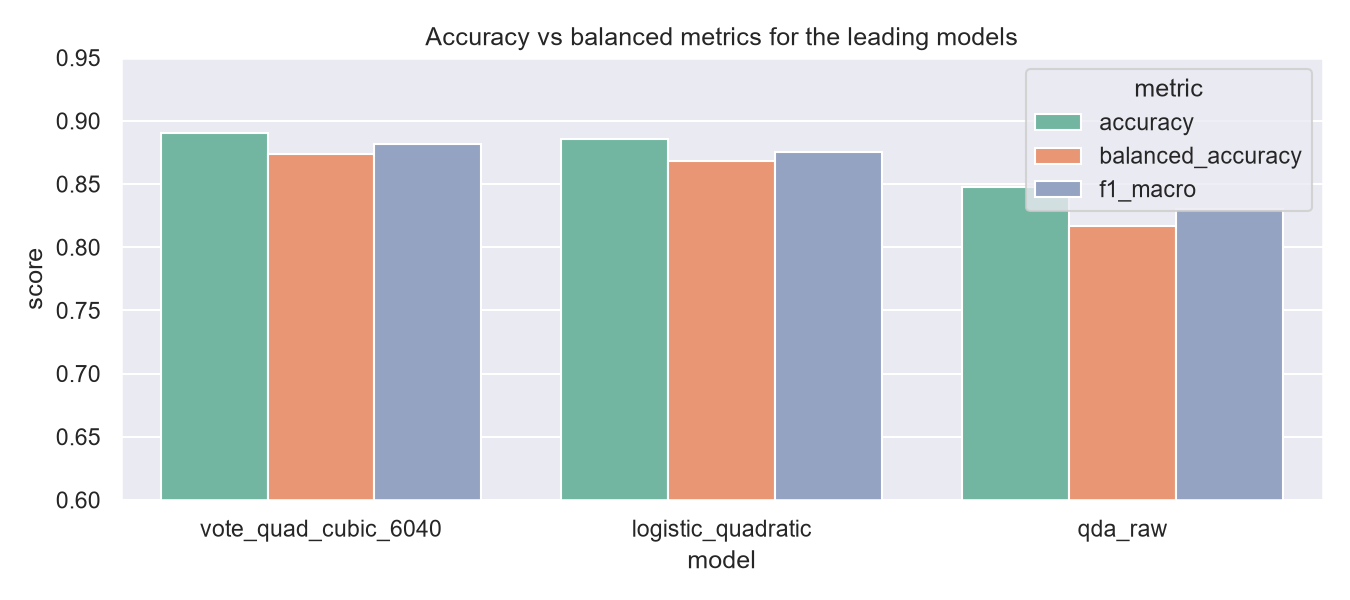
\includegraphics[width=\linewidth]{machine_balanced_metrics.png}
  \caption{accuracy vs balanced metrics}
\end{subfigure}
\caption{Discrimination and class-balance checks.}
\label{fig:machbal}
\end{figure}

\paragraph{t-SNE.} We also draw a t-SNE projection of a 3,000-row sample, before and after feature engineering (Figure~\ref{fig:tsne}), as an illustration of how the classes are present relative to each other. On the raw sensors the three classes form broad overlapping clouds, with mechanical machines mostly in the upper region and thermal machines largely on the right. After adding the engineered features the thermal cloud becomes smaller on the right and the mechanical group separates more cleanly from the normal machines in the middle.

\begin{figure}[H]
\centering
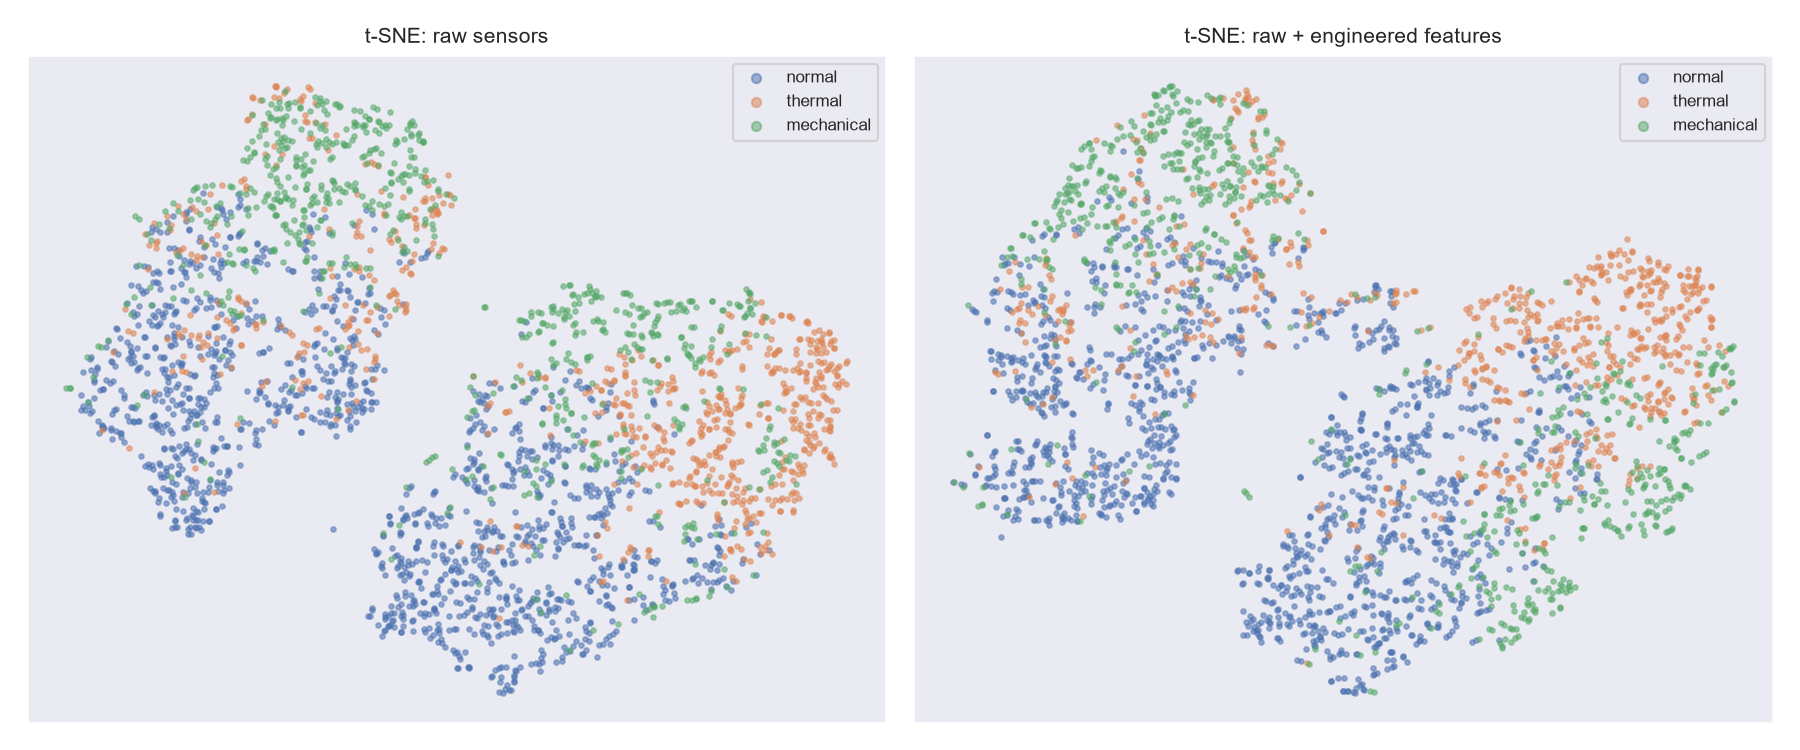
\includegraphics[width=\linewidth]{machine_tsne_before_after.png}
\caption{t-SNE before and after feature engineering.}
\label{fig:tsne}
\end{figure}

\section{Cross-validation of shortlisted models}

Since a single 5-fold estimate can change with the fold split chosen, we re-evaluate the three best models with 5 folds repeated 3 times: the quadratic logistic regression (0.8853 $\pm$ 0.0056), the random forest (0.8777 $\pm$ 0.0051) and QDA (0.8476 $\pm$ 0.0068). We checked the same for the ensembled model (60/40 voting based) in the 80/20 test above.

\section{Metrics comparison}

We finally evaluate one representative configuration per family under accuracy, balanced accuracy and macro $F_1$.

\begin{table}[H]
\centering
\small
\setlength{\tabcolsep}{5pt}
\begin{tabular}{@{}>{\raggedright\arraybackslash}p{6.4cm}rrr@{}}
\toprule
Model & Accuracy & Balanced acc. & Macro $F_1$ \\
\midrule
Logistic regression, quadratic basis (deg 2, $C=1$) & 0.8853 & 0.8681 & 0.8756 \\
Random forest (depth 14) & 0.8787 & 0.8554 & 0.8655 \\
QDA (raw sensors, reg 0.1) & 0.8476 & 0.8171 & 0.8299 \\
Decision tree, cost-complexity pruned & 0.8429 & 0.8194 & 0.8259 \\
Decision tree, pre-pruned (depth 12, leaf 5) & 0.8389 & 0.8126 & 0.8206 \\
Logistic regression, linear ($C=10$) & 0.8293 & 0.8037 & 0.8104 \\
LDA & 0.8239 & 0.7893 & 0.8022 \\
Gaussian naive Bayes (smoothing 0.1) & 0.7535 & 0.7244 & 0.7273 \\
\bottomrule
\end{tabular}
\caption{Machine condition: full metrics comparison.}
\end{table}

From the table above, we see that the quadratic logistic regression leads on all three metrics among the single models, the random forest follows closely, the post-pruned tree is the best tree, and Gaussian Naive Bayes performed the worst. The ensemble model based on the 60/40 voting is ahead of every other model (0.8901 accuracy).

\section{Submission CSV Creation and Best Model Choice}

For the submissions, we fit every model on all training rows and write one CSV per model.

\begin{table}[H]
\centering
\caption{Best model and its submission.}
\label{tab:final}
\small
\begin{tabular}{@{}>{\raggedright\arraybackslash}p{4.9cm}cc>{\raggedright\arraybackslash}p{3.1cm}@{}}
\toprule
Final model & CV score & Public LB & Submission file \\
\midrule
Soft vote of quadratic (60\%) and cubic (40\%) logistic & acc 0.8901 & 0.89125 & \texttt{submission.csv} \\
\bottomrule
\end{tabular}
\end{table}

The public leaderboard scores on Kaggle were: quadratic logistic 0.88812, cubic logistic 0.88687, random forest 0.88125, QDA 0.85625 and the post-pruned tree 0.84937. We checked the scores for the ensemble models in previous sections (higher than all of these).

\section{Conclusion}

\begin{itemize}
  \item Even though the failure types are unevenly distributed (a 2:1:1 split), our accuracy metric isn't masking poor performance on a minority class. We could observe that seeing the lowest recall was 83.3\% for thermal failures, and our top model also led on accuracy, balanced accuracy and macro $F_1$.
  \item The raw sensor data separates the failure types in the same way that they logically and physically should, and our custom engineered features made the boundaries between them definite.
  \item The decision boundaries between the machine states are curved. Hence, upgrading standard logistic regression with degree-2 polynomial features increased the accuracy from 0.829 to 0.885, better than both QDA (0.848) and the random forest (0.879); a cubic basis with stronger regularisation reached even higher accuracy (0.889).
  \item When tuning the decision trees, we tested both pruning methods: setting limits beforehand (pre) (max depth 12, minimum leaf size 5) gave a maximum of 0.839 accuracy, while cost-complexity (post-)pruning increased that further to 0.842.
  \item We tried handling the class imbalance with class reweighting, oversampling and SMOTE, but all of them were detrimental to the performance metrics.
  \item Finally, the best-performing model was the 60/40 combination (with soft voting) of the quadratic and cubic logistic regressions: 0.8901 accuracy in cross-validation, and 0.89125 on the public leaderboard for the industrial machine condition classification competition on Kaggle.
\end{itemize}

\end{document}
